\begin{solution}
\begin{enumerate}
\item The first row of this operator matrix differential equation gives 
      \[ u_t(x,t) = v(x,t),\]
      which is simply the definition of $v$.  The second row gives
      \[ v_t(x,t) = u_{xx}(x,t) - 2d v(x,t).\]
      Substituting in our definition $v=u_t$ (and hence $v_t = u_{tt}$),
      we obtain
      \[ u_{tt}(x,t) = u_{xx}(x,t) - 2d u_t(x,t),\]
      which is the damped wave equation.

\item Multiply $A(d)$ against $\Psi_{\pm k}$ to obtain
\begin{eqnarray*}
 \bmatrix{ 0 & I \cr \partial^2/\partial x^2 & -2@d@I}
    \bmatrix{ \sin(k \pi x)\cr  \lambda_{\pm k} \sin(k\pi x)} 
    &=& \bmatrix{ \lambda_{\pm k}\sin(k \pi x)\cr  (d^2/dx^2)(\sin(k\pi x)) - 2d\lambda_{\pm k} \sin(k\pi x)} \\[0.5em]
    &=& \bmatrix{ \lambda_{\pm k}\sin(k \pi x)\cr  -k^2\pi^2 \sin(k\pi x)) - 2d\lambda_{\pm k} \sin(k\pi x)}.
\end{eqnarray*}
We want this vector to be of the form
\[ \lambda_{\pm k}\bmatrix{ \sin(k \pi x)\cr  \lambda_{\pm k} \sin(k\pi x)};\]
the first component is already in the correct form, but the second component
requires that
\[ -k^2\pi^2 - 2d \lambda_{\pm k} = \lambda_{\pm k}^2.\]
That is, we must solve the quadratic equation
\[ \lambda_{\pm k}^2 +2d \lambda_{\pm k} +k^2\pi^2 = 0,\]
which, via the quadratic formula, gives
\[ \lambda_{\pm k} = -d \pm \sqrt{d^2 - k^2\pi^2}.\]
(It is no coincidence that these are the values that appear in the exponential
in the solution $a_k(t)$ to the ODE in the previous problem!)

\item The eigenvalues for $d = 0, \pi/2, \pi, 3\pi/2$ are plotted below.

\begin{center}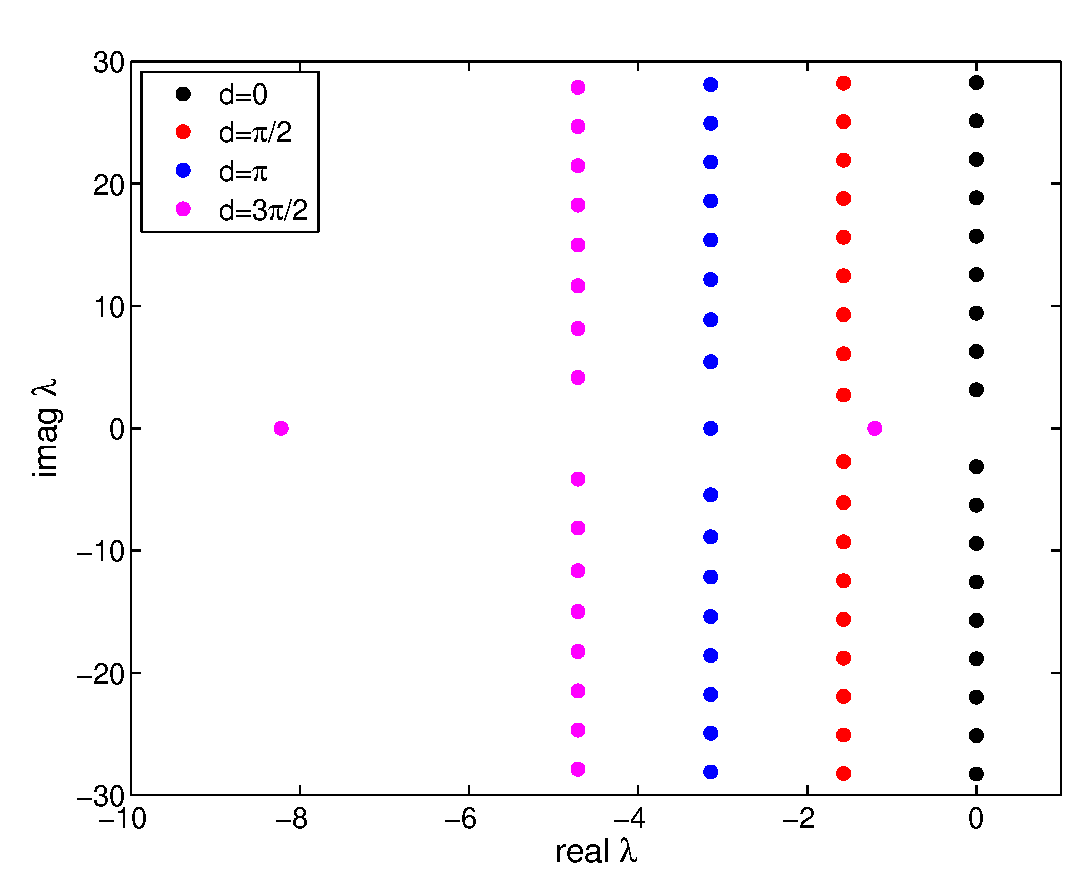
\includegraphics[scale=0.6]{optdamp1}\end{center}

{\small\begin{verbatim}
 d = [0 pi/2 pi 3*pi/2];
 col = 'krbm'
 k = 1:10;
 figure(1), clf
 for j=1:length(d)
     ew = [-d(j)+sqrt(d(j)^2-k.^2*pi^2) -d(j)-sqrt(d(j)^2-k.^2*pi^2)];
     plot(real(ew),imag(ew),'.','markersize',20,'color',col(j)), hold on
 end
 axis([-10 1 -30 30]) 
 set(gca,'fontsize',14)
 xlabel('real \lambda','fontsize',16)
 ylabel('imag \lambda','fontsize',16)
 legend('d=0','d=\pi/2','d=\pi','d=3\pi/2',2)
 print -depsc2 optdamp1
\end{verbatim}}

\item For $d \in [0,\pi]$, the eigenvalues $\lambda_{\pm k}$ will all
      fall on a vertical line in the complex plane with real part $-d$.
      When $d=\pi$, we have a double eigenvalue, $\lambda_{\pm 1} = -\pi$,
      and for $d>\pi$, we will always have a real rightmost eigenvalue of
          \[ \lambda_{+1} = -d + \sqrt{d^2-\pi^2}.\]
      Taking a derivative with respect to $d$, we have for $d>\pi$,
          \[ \lambda_{+1}' = -1 +{d \over \sqrt{d^2-\pi^2}}
                           = -1 +{1 \over \sqrt{1-\pi^2/d^2}} > 0,\]
     and thus we conclude that 
     \[ d= \pi\]
     maximizes the real part of the rightmost eigenvalue, and hence the 
     energy decay rate of the system.  (It takes some careful mathematics to  
     show that the rightmost eigenvalue determines the energy decay rate in
     this infinite dimensional system; this was accomplished in a 1994 paper by
     S. J. Cox and E. Zuazua.)

     [GRADERS: Students can receive full credit for solutions that are less
     rigorous than the one presented here.]

\item The solutions for $d=2.5$, $3.2$, and $20$ at time $t=1.5$ are shown
     in the plot below.  Note that despite the large damping term at $d=20$,
     the solution remains large.  We say that the system is \emph{overdamped}.
     Near optimal damping, $d\approx \pi$, we can smaller solutions.

\begin{center}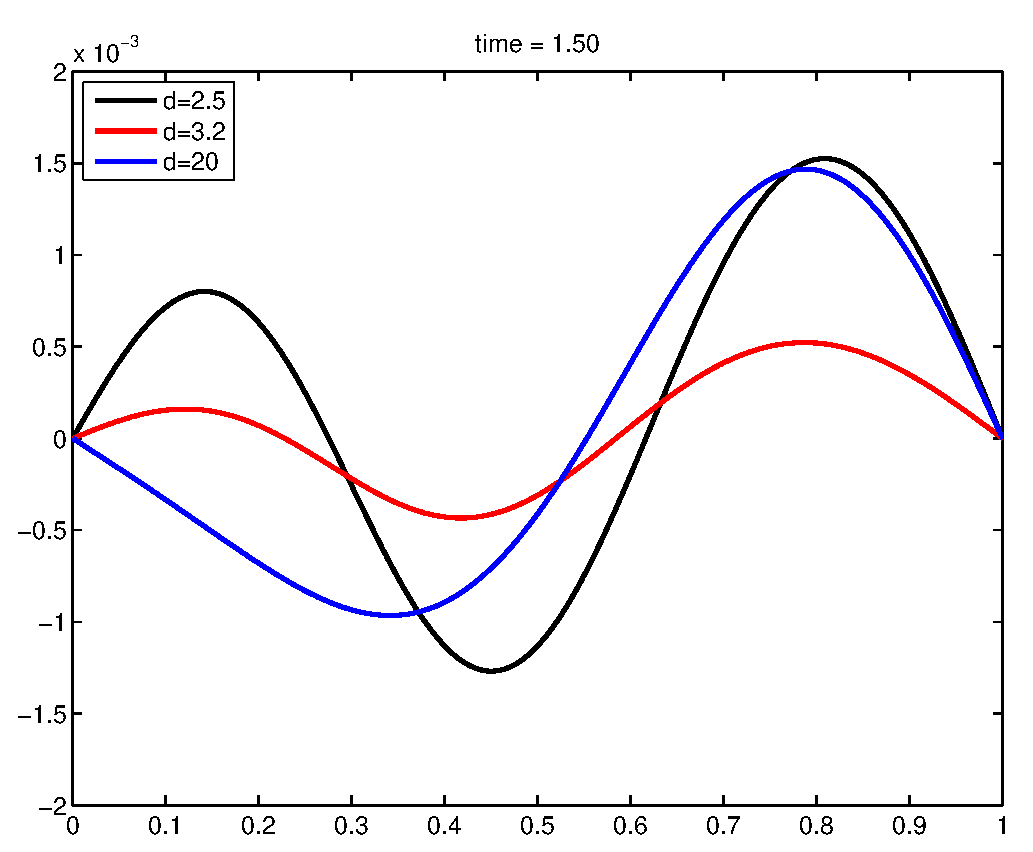
\includegraphics[scale=0.6]{optdamp2}\end{center}

{\small \begin{verbatim}
 t = 1.5;
 dvec = [2.5 3.2 20];
 xx = linspace(0,1,500)';

 ak0 = zeros(10,1);
 bk0 = zeros(10,1);
 k = [1:20]';
 bk0 = -6*sqrt(2)*(1+(-1).^k).*k./((k.^2-9).^2*pi^2);
 bk0(3) = sqrt(2)/4;

 figure(1), clf
 cvec = 'krb';
 for m=1:length(dvec)
    d = dvec(m)
    u = zeros(size(xx));
    for k=1:length(bk0)
        psik = sqrt(2)*sin(k*pi*xx);
        dis = sqrt(d^2-k^2*pi^2);
        ak = bk0(k)*(exp((-d+dis)*t)-exp((-d-dis)*t))/(2*dis);
        u = u+ak*psik;
    end 
    plot(xx,u,'-','linewidth',2,'color',cvec(m)), hold on
    ylim([-.002 .002])
    title(sprintf('time = %3.2f', t))
 end
 legend('d=2.5','d=3.2','d=20',2)
 print -depsc2 optdamp2
\end{verbatim}}
\end{enumerate}
\end{solution}
